\documentclass[fontsize=12pt,a4paper]{scrartcl}
 
\usepackage[T1]{fontenc}    
\usepackage[latin1]{inputenc} 
 
\usepackage{textcomp} 
\usepackage{amsmath}
\usepackage{amssymb}
\usepackage{graphicx}
\usepackage{listings}
\lstset{tabsize=4, showspaces=false}


\title{Machine Learning SS2013}
\subtitle{Ulrike von Luxburg \\ Assignment 06}
\author{Arne Schr�der \and Falk Oswald \and Angel Bakardzhiev}
 
\date{\today} 
 
\begin{document}
\maketitle

 \section*{Exercise 1}
    \begin{figure}[h!]
        \centering
        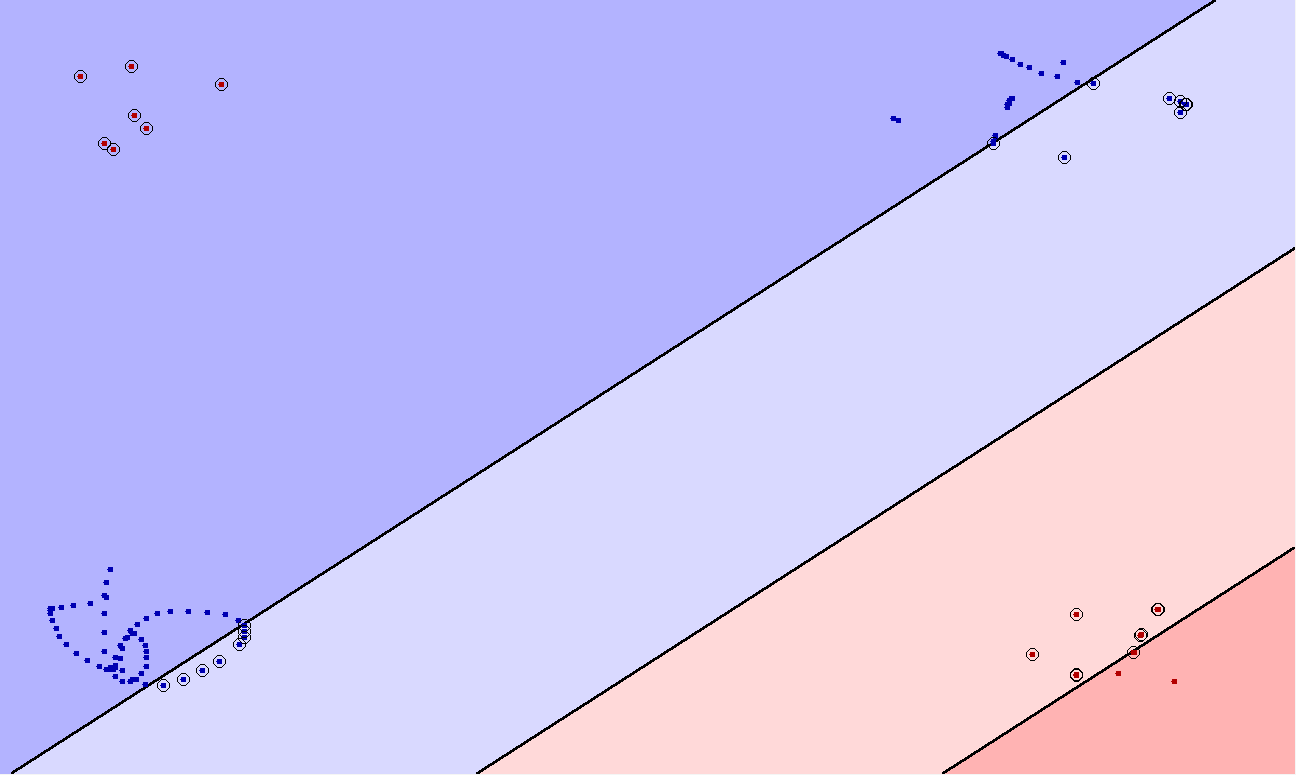
\includegraphics[width=0.9\textwidth]{linear_c100.PNG}
        \caption{Linear kernel with $C = 100$}
    \end{figure}

    \begin{figure}[h!]
        \centering
        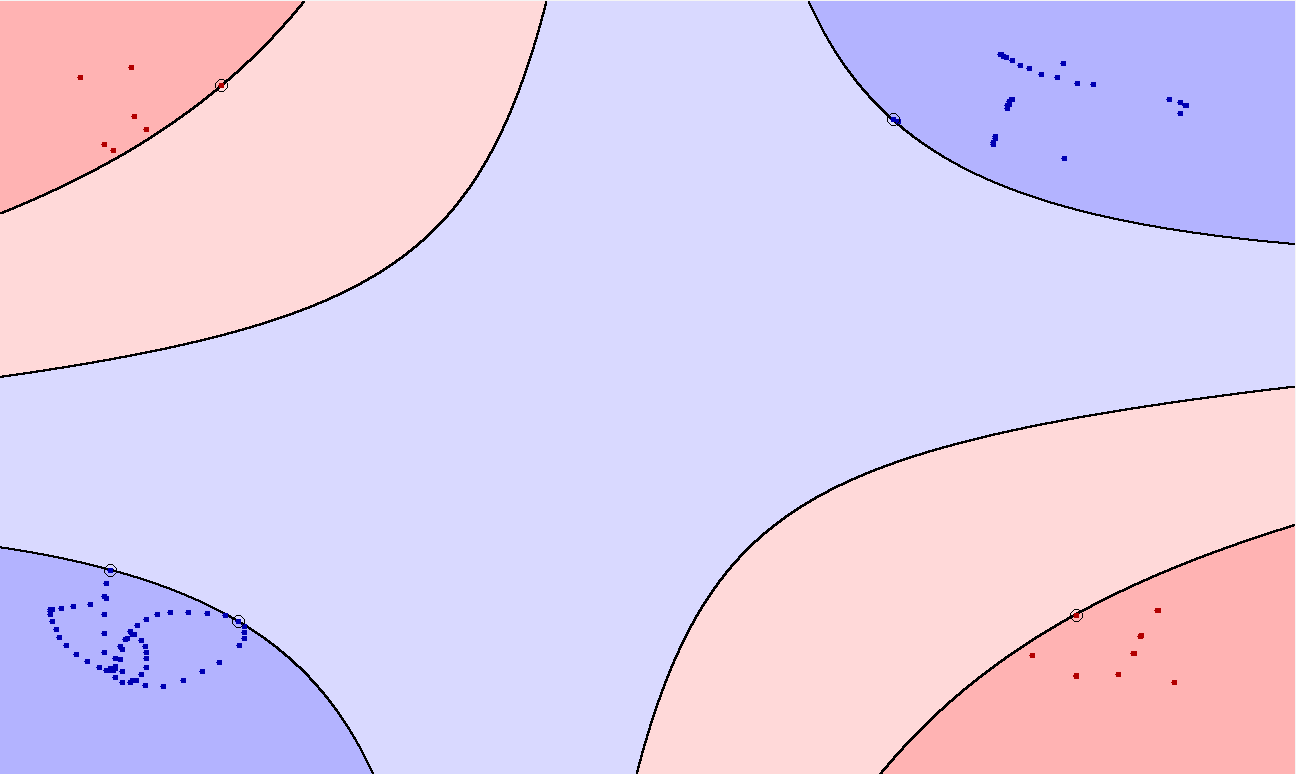
\includegraphics[width=0.9\textwidth]{polynomial_d2_c100.PNG}
        \caption{Polynomial kernel with $d = 2$ and $C = 100$}
    \end{figure}

    \begin{figure}[h!]
        \centering
        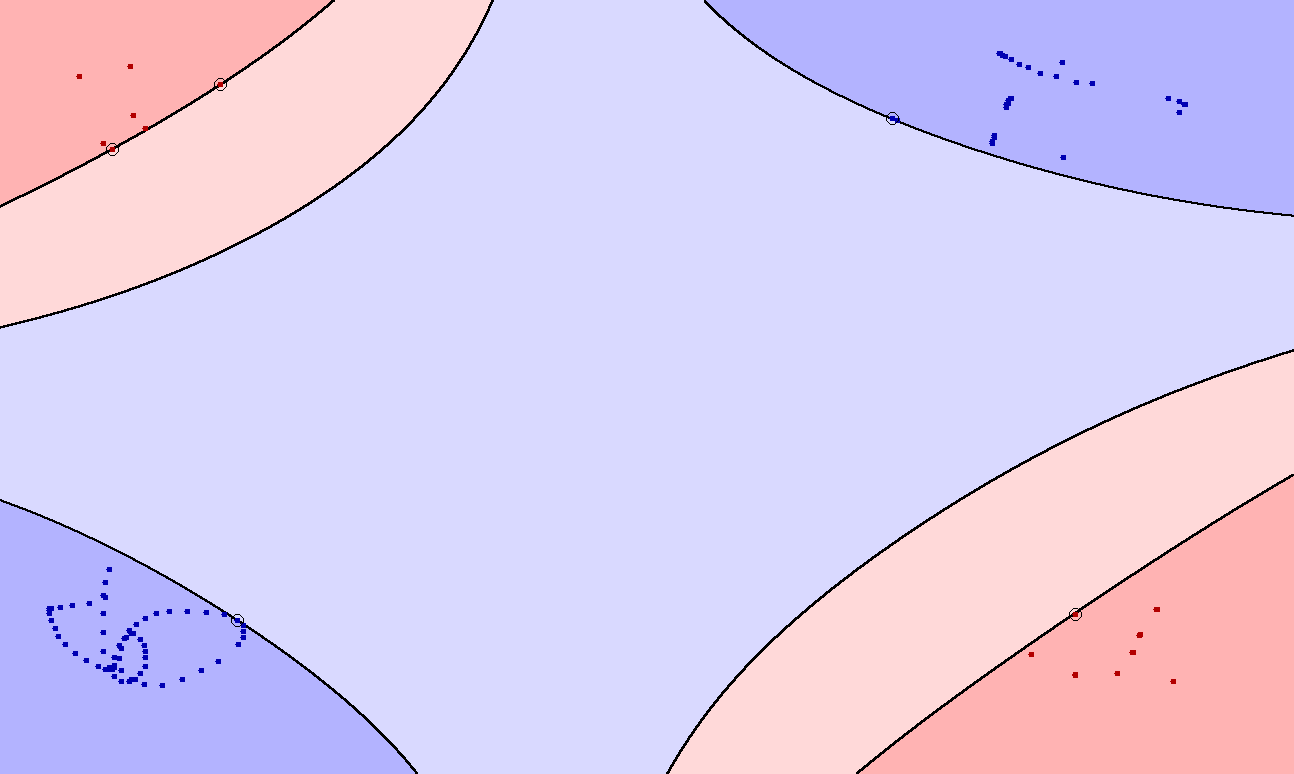
\includegraphics[width=0.9\textwidth]{polynomial_d7_c100.PNG}
        \caption{Polynomial kernel with $d = 7$ as 8 was not available and $C = 100$}
    \end{figure}

    \begin{figure}[h!]
        \centering
        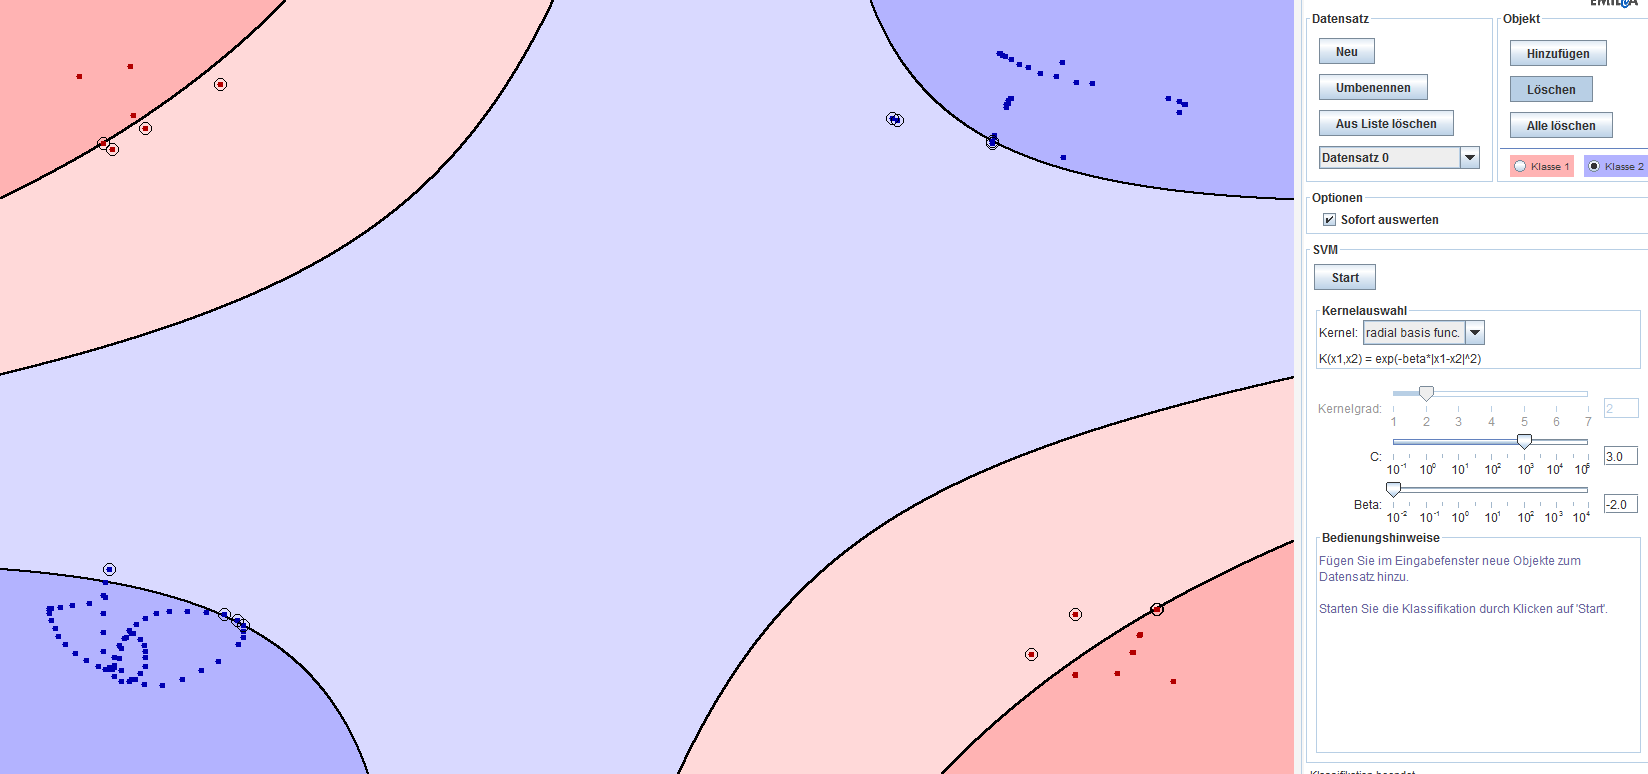
\includegraphics[width=0.9\textwidth]{rbf_b001_c1000.PNG}
        \caption{Gaussian kernel with $\beta = 10^{-2}$ and $C = 1000$}
    \end{figure}

    \begin{figure}[h!]
        \centering
        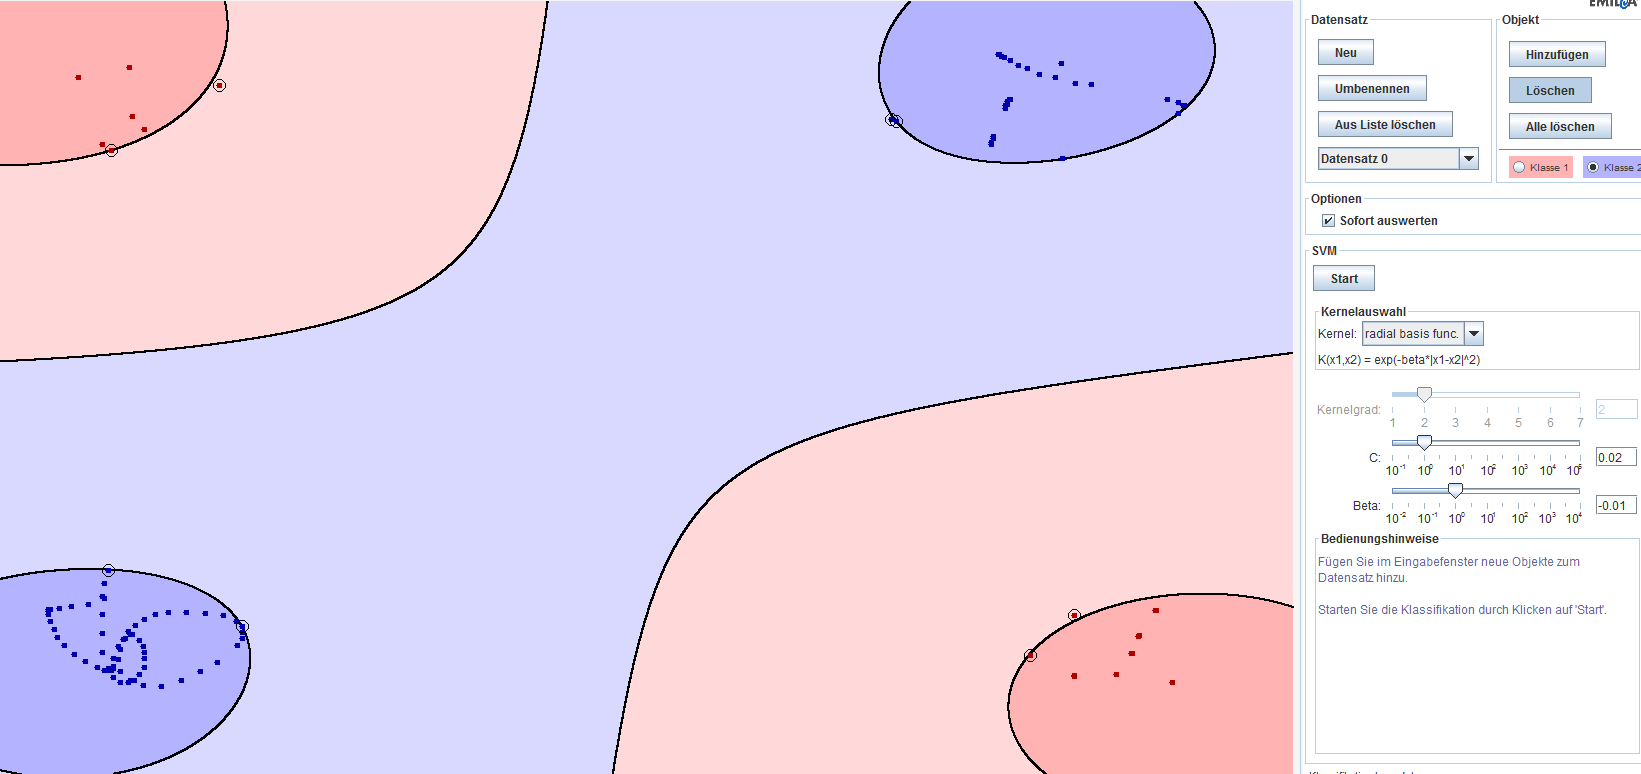
\includegraphics[width=0.9\textwidth]{rbf_b1_c1.PNG}
        \caption{Gaussian kernel with $\beta = 10^{0}$ and $C = 1$}
    \end{figure}

    \begin{figure}[h!]
        \centering
        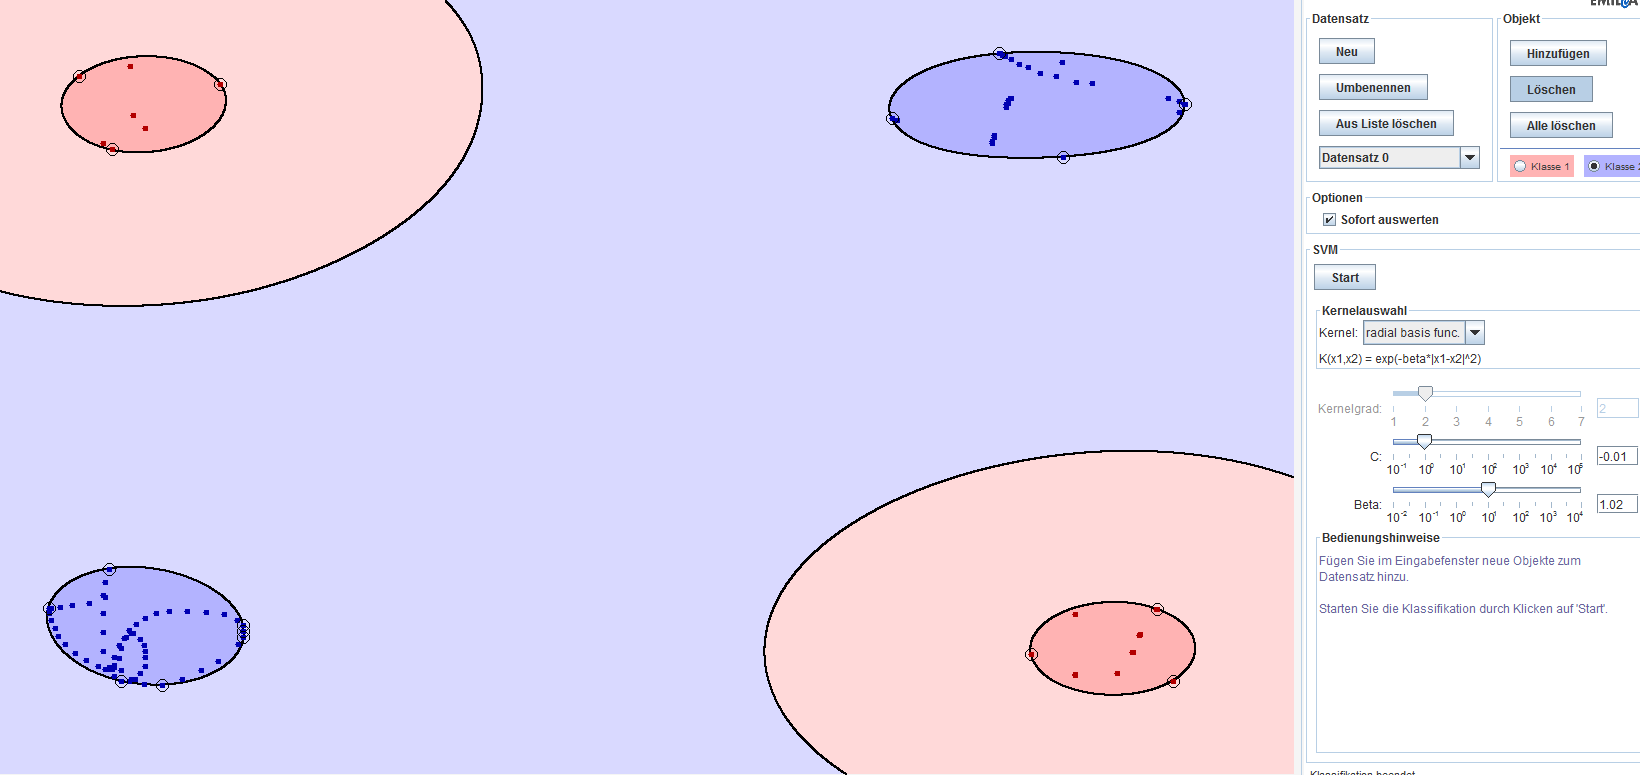
\includegraphics[width=0.9\textwidth]{rbf_b10_c1.PNG}
        \caption{Gaussian kernel with $\beta = 10^{1}$ and $C = 1$}
    \end{figure}

    \begin{figure}[h!]
        \centering
        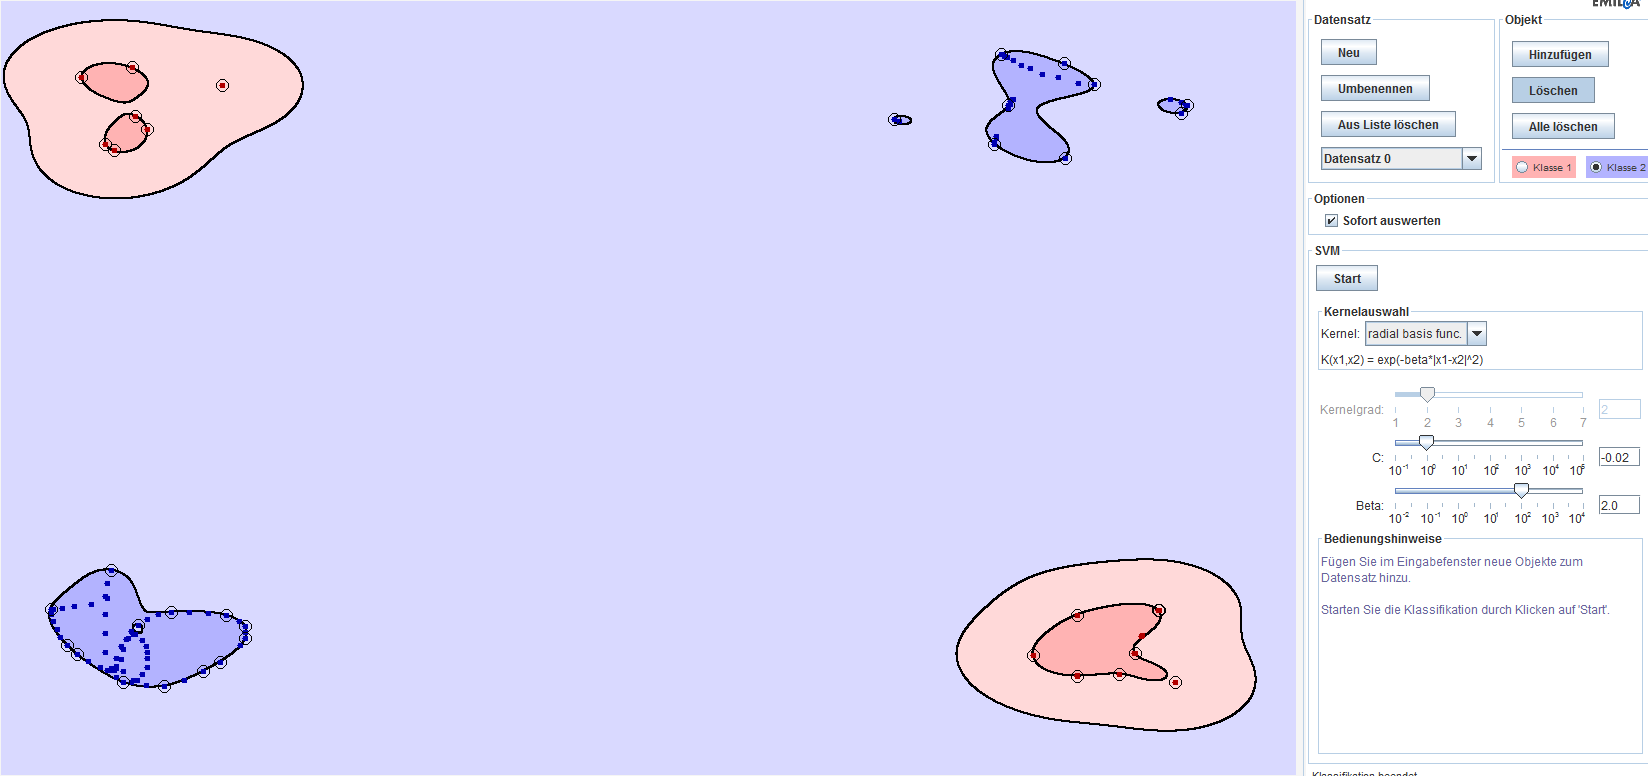
\includegraphics[width=0.9\textwidth]{rbf_b100_c1.PNG}
        \caption{Gaussian kernel with $\beta = 10^{2}$ and $C = 1$}
    \end{figure}

    \begin{figure}[h!]
        \centering
        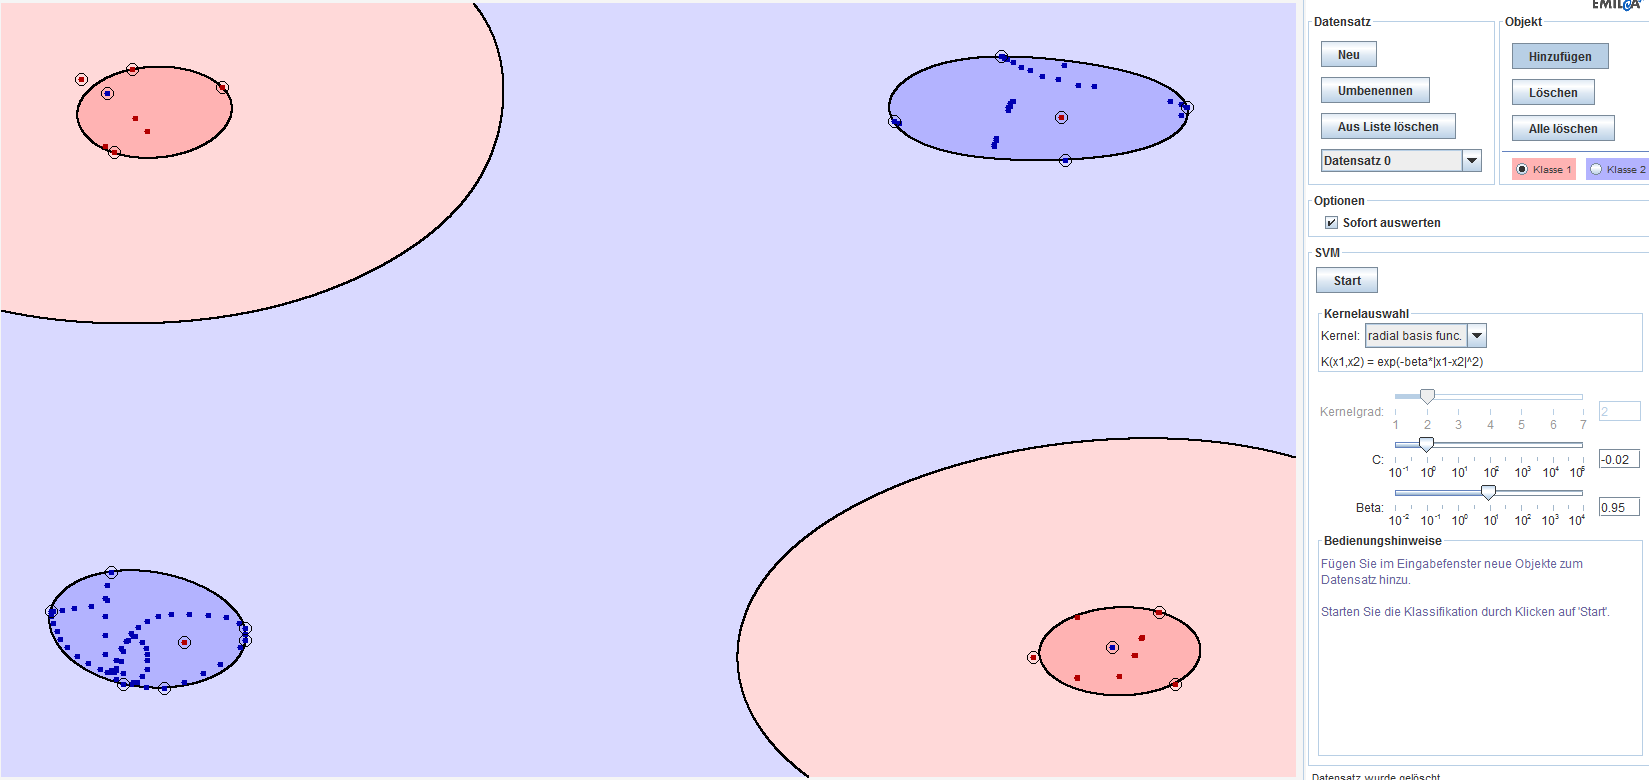
\includegraphics[width=0.9\textwidth]{noise_rbf_b10_c1.PNG}
        \caption{Gaussian kernel with noise and $\beta = 10$ and $C = 1$ as 0 was not available}
    \end{figure}

    \begin{figure}[h!]
        \centering
        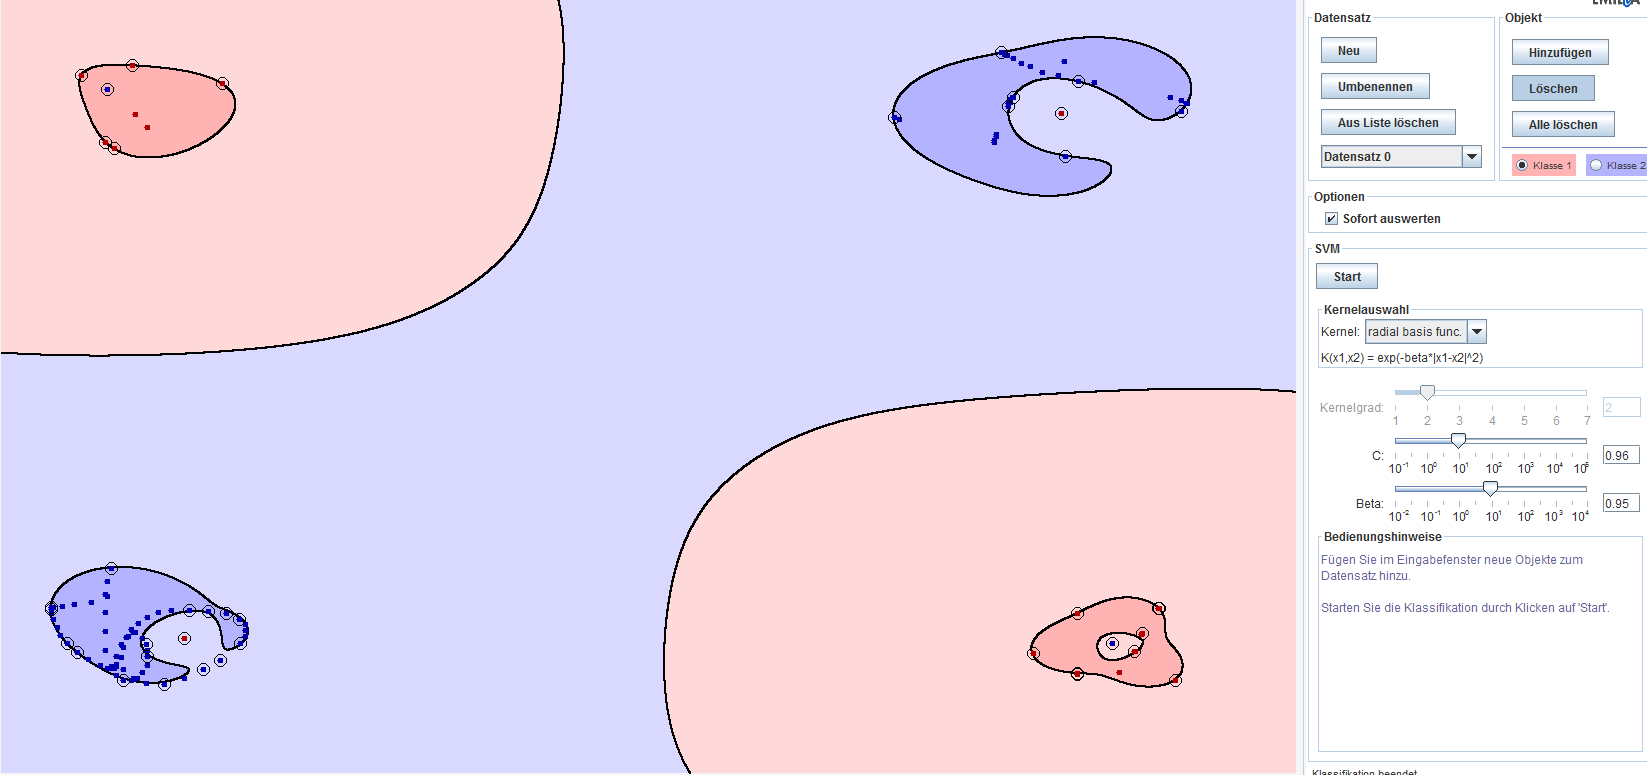
\includegraphics[width=0.9\textwidth]{noise_rbf_b10_c10.PNG}
        \caption{Gaussian kernel with noise and $\beta = 10$ and $C = 10$}
    \end{figure}

    \begin{figure}[h!]
        \centering
        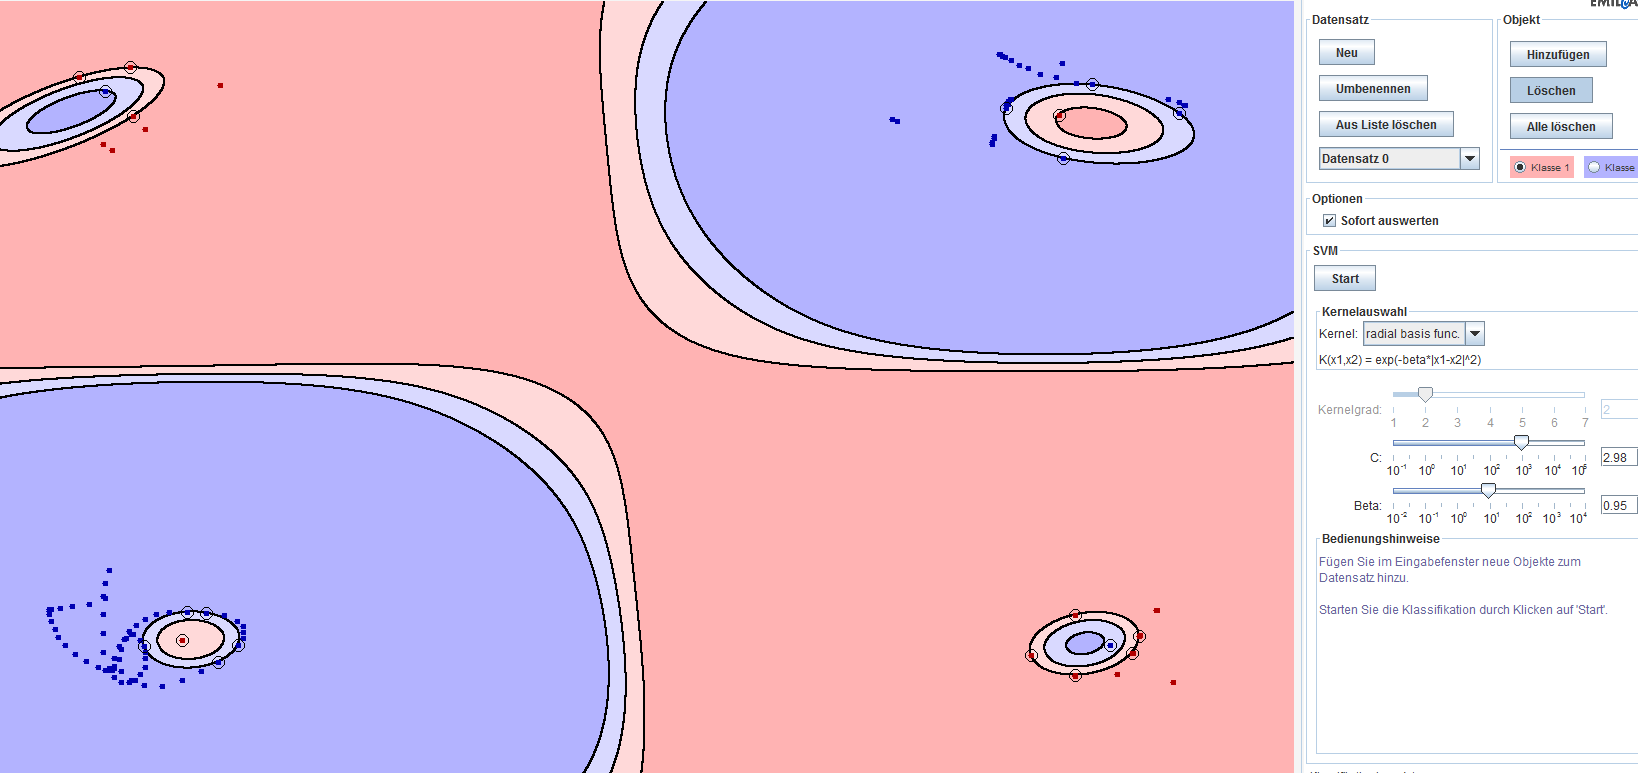
\includegraphics[width=0.9\textwidth]{noise_rbf_b10_c1000.PNG}
        \caption{Gaussian kernel with noise and $\beta = 10$ and $C = 1000$}
    \end{figure}

	The best choice of parameters for the example with noise is $C=1$.

\newpage
\mbox{}
\newpage
\mbox{}
\newpage
\mbox{}
\newpage
\mbox{}
\newpage

 \section*{Exercise 2}
    Figure 2 a from the assignment sheet is most likely to be a Gaussian kernel (rbf) with parameters $\beta = 10$.
	
	One could argue, that this scenario is already overfitting as a linear kernel would only lead to two false positives but a much simpler solution. On the other hand, the Gaussian kernel does classify every point correctly and provides a not too complex function. A change in parameters is not essentially neccesary.
	
	Figure 2 b is most likely to be a polynomial kernel with parameter $c = 10$.
	
	The chosen scenario does not separate the classes correctly. Points, which are most definitely no outliers (as they lie in groups) are classified wrong. The situation can be made better by raising $c$ to 100 and the degree $d$ to 3.
	
	We guess that almost all points are support vectors. Maybe some of the points inbetween other points of the same class are not.
	
\section*{Exercise 3}

\subsection*{Task}
Write the primal and dual of SVM in matrix form.

\subsection*{Solution}

Soft margin linear SVM: Primal:

\begin{align*}
\min_{w, \xi b} \quad \frac{1}{2} w^T \cdot w + \frac{C}{n} \xi^T \cdot \mathbb{1}_n \\
y_i(w^T x_i + b) \geq 1 - \xi_i \quad i = 1, \dots, n \\
\xi_i \geq 0 \quad i = 1, \dots, n
\end{align*}

Dual:

\begin{align*}
\max_\alpha \alpha^T \cdot \mathbb{1}_n - \frac{1}{2} \alpha^T \\
\alpha Y = 0 \\
0 \leq \alpha_i \leq \frac{C}{n} \qquad i = 1, \dots, n
\end{align*}

Kernel SVM: Primal:

\begin{align*}
\min_{w, \xi b} \quad \frac{1}{2} \beta^T K \beta + \frac{C}{n} \xi^T \cdot \mathbb{1}_n \\
y_i(w^T \Phi(x_i) + b) \geq 1 - \xi_i \quad i = 1, \dots, n \\
\xi_i \geq 0 \quad i = 1, \dots, n
\end{align*}

Dual:

\begin{align*}
\max_\alpha \alpha^T \cdot \mathbb{1}_n - \frac{1}{2} \alpha^T \\
\alpha Y = 0 \\
0 \leq \alpha_i \leq \frac{C}{n} \qquad i = 1, \dots, n
\end{align*}

\section*{Exercise 4}
Assume that $K1;K2 : \mathcal{X} \times \mathcal{X} \rightarrow \mathbb{R} $ are kernel functions. Which of the following functions are also a valid kernel? Prove or bring a counterexample.

A kernel function is defined as:\\
\[ \sum_{i,j=1}^n c_i c_j k(x_i,x_j) \geq 0  \] 
with $ x_i \in \mathcal{X}$, $c_1,...,c_n \in \mathbb{R}$, $n\geq 1$
\subsection*{a) $K = \alpha K_1 \ for \ \alpha \geq 0$ }
For the general kernel function we insert $\alpha K_1$ and move $\alpha$ in front of the sum.
\[\sum_{i,j=1}^n c_i c_j \alpha K_1(x_i,x_j) = \alpha \underbrace{\sum_{i,j=1}^n c_i c_j K_1(x_i,x_j)}_{\geq 0}   \]
As $\alpha \geq 0$ and $K_1 \geq 0$, is K a valid kernel.

\subsection*{b) $K = K_1 + K_2$}
We want to show that $\sum_{i,j=1}^n c_i c_j K(x_i,x_j) \geq 0$:
\begin{align*}
\sum_{i,j=1}^n c_i c_j K(x_i,x_j) &= \sum_{i,j=1}^n c_i c_j (K_1(x_i,x_j) + K_2(x_i,x_j))\\
&=  \sum_{i,j=1}^n c_i c_j K_1(x_i,x_j) + \sum_{i,j=1}^n c_i c_j K_2(x_i,x_j) \geq 0
\end{align*}

As $K_1$ and $K_2$ are valid kernels, 
$ \sum_{i,j=1}^n c_i c_j K_1(x_i,x_j) \geq 0 $ and $ \sum_{i,j=1}^n c_i c_j K_2(x_i,x_j) \geq 0 $ holds.

\subsection*{c) $K = K_1 - K_2$}
We want to show that $\sum_{i,j=1}^n c_i c_j K(x_i,x_j) < 0$

We choose 
\begin{align*}
& K_1:(x,y) \mapsto \langle x,y \rangle \\
& K_2 = 2 \cdot K_1
\end{align*}

With 
\begin{align*}
\sum_{i,j=1}^n c_i c_j K_1(x_i,x_j) - \sum_{i,j=1}^n c_i c_j K_2 (x_i,x_j) &= \sum_{i,j=1}^n c_i c_j (K_1(x_i,x_j) - K_2(x_i, x_j))\\
&= \sum_{i,j=1}^n c_i c_j -K_1(x_i,x_j)\\
&= - \underbrace{\sum_{i,j=1}^n c_i c_j K_1(x_i,x_j)}_{\geq 0}\\
\end{align*}
We have to show that for one $n,x,c$ the expression $-\sum_{i,j=1}^n c_i c_j K_1(x_i,x_j)$ can be negative.

We choose  $ \mathcal{X}=\mathbb{R}, n=1, x_1=1, c_1=1$:
\begin{align*}
-\sum_{i,j=1}^1 c_i c_j K_1(x_i,x_j) &= - c_1^2 \cdot  K_1(x_i,x_j)\\
&= - 1 \cdot 1 < 0
\end{align*}

\subsection*{e) $K(x,y) = f(x)K_1(x,y)f(y) $ for any function $f:\mathcal{X} \rightarrow \mathbb{R}$ }

\section{Exercise 5}
We want to show that $ \sum_{i,j=1}^n c_i c_j K(x_i,x_j) \geq 0$.\\
With $K(x,y):=f(x)K_1(x,y)f(y)$ we have 
\begin{align*}
\sum_{i,j=1}^n c_i c_j K(x_i,x_j) &= \sum_{i,j=1}^n c_i c_j f(x_i)K_1(x_i,x_j)f(x_i) \\
&= \sum_{i,j=1}^n c_i f(x_i) c_j f(x_j)K_1(x_i,x_j)
\end{align*}

Now we choose $c_i' = c_i \cdot f(x_i), c_j' = c_j \cdot f(x_j)$ and have
\[ \sum_{i,j=1}^n c_i' c_j' K_1(x_i,x_j) \geq 0 \]

\subsection*{Task 1}

Show that the corresponding feature map $\Phi$ is given by $\Phi(x) = (1, \sqrt{2} x_1, \sqrt{2} x_2, x_1^2, x_2^2, \sqrt{2} x_1 x_2)^T$.

\subsection*{Solution}

\begin{align*}
  \langle \Phi(x), \Phi(y) \rangle & = \langle (1, \sqrt{2} x_1, \sqrt{2} x_2, x_1^2, x_2^2, \sqrt{2} x_1 x_2)^T, (1, \sqrt{2} y_1, \sqrt{2} y_2, y_1^2, y_2^2, \sqrt{2} y_1 y_2)^T \rangle \\
  & = (1, \sqrt{2} x_1, \sqrt{2} x_2, x_1^2, x_2^2, \sqrt{2} x_1 x_2) \cdot (1, \sqrt{2} y_1, \sqrt{2} y_2, y_1^2, y_2^2, \sqrt{2} y_1 y_2)^T \\
  & = 1 + 2 x_1 y_1 + 2 x_2 y_2 + x_1^2 y_1^2 + x_2^2 y_2^2 + 2 x_1 y_1 x_2 y_2 \\
  & = (x_1 y_1 + x_2 y_2 + 1)^2 = (x^T y + 1)^2 = K(x, y)
\end{align*}

\subsection*{Question}

If we use the second degree polynomial kernel for inputs from $\mathbb{R}^d$, what would be the dimensionality of the corresponding feature space?

\subsection*{Answer}

For $x, y \in \mathbb{R}^d$ the product $x^T y$ results in a sum of $d$ terms. Therefore $(x^T y + 1)$ results in a sum of $d + 1$ terms. This means that for the square there are going to be $\frac{(d+1)(d+2)}{2}$ terms, which will all need to be represented in the feature space. Therefore, the feature space is going to be of dimension $\frac{(d+1)(d+2)}{2}$.
 \end{document}
